\documentclass[10pt]{article}
\usepackage{icmlko}

\icmlmeta{IP 파운데이션 월드모델}{32}{문턱은 눈금보다 비싸다}{눈금은 여덟 건이면 되는데 문턱 판정은 쉰 건이 필요하다}

\begin{document}

\twocolumn[
\icmlheader

\begin{abstract}
노트 31은 절대량 단계로 넘어갈 실무 문턱을 순위 상관 r$\geq$0.5로 잡았다. 실전에서
그 판정을 하려면 대상 도메인 라벨 k건으로 상관을 추정해야 한다. 몇 건이 필요한지
쟀다. \textbf{추정 자체는 거의 편향이 없다} --- 팝업 참값 $+$0.445에 대해 k=8에서
$+$0.42, k=50에서 $+$0.45다. 표준편차만 k에 따라 줄어든다(0.32 $\to$ 0.07).
\textbf{그런데 문턱 판정 정확도는 훨씬 늦게 오른다.} k=8에서 세 도메인 모두
56--57\%로 동전 던지기 수준이고, k=20에서 63--74\%, k=50에서야 78--96\%가 된다.
가장 어려운 것은 팝업이다 --- 참값 $+$0.445가 문턱 0.5에 가까워 k=50에서도
78\%에 그친다. \textbf{눈금 보정은 여덟 건, 문턱 판정은 쉰 건.} 같은 파이프라인
안에서 필요한 라벨이 여섯 배 차이 난다. 그리고 이 비대칭은 절차의 순서를 바꾼다
--- 문턱을 사전에 확정하려 하면 절대량 자체보다 비싸지므로, 보수적 하한으로
판정하거나 사후 검증으로 돌리는 편이 낫다.
\end{abstract}
]

\section{문턱을 실전에서 쓰려면}

노트 31은 순위 상관이 절대량의 성패를 정한다는 것을 보이고 r$\geq$0.5를 실무
문턱으로 제시했다. 그런데 그 상관은 \emph{전량 라벨}로 쟀다. 새 도메인에서는
라벨이 없으므로 k건으로 추정해야 한다.

노트 21이 눈금 보정에 8--20건이면 된다고 했으니 문턱 판정도 비슷할 것이라
짐작했다. 재봤다.

\section{추정은 정확한데 판정은 아니다}

\begin{figure}[t]
\centering
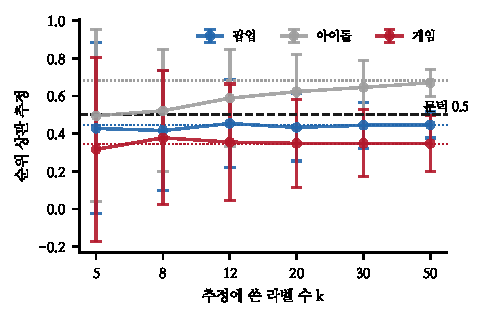
\includegraphics[width=\columnwidth]{figs/sd.pdf}
\caption{k건으로 추정한 순위 상관. 점선이 각 도메인의 참값, 굵은 파선이 문턱이다.}
\end{figure}

\begin{table}[t]
\centering\tsize
\caption{순위 상관 추정. 400회 반복 평균 $\pm$ 표준편차.}
\begin{tabular}{lrrrr}
\toprule
도메인 & 참 r & k=8 & k=20 & k=50 \\
\midrule
팝업 & $+$0.445 & $+$0.42 $\pm$ .32 & $+$0.43 $\pm$ .18 & $+$0.45 $\pm$ .07 \\
아이돌 & $+$0.681 & $+$0.52 $\pm$ .32 & $+$0.62 $\pm$ .19 & $+$0.67 $\pm$ .07 \\
게임 & $+$0.344 & $+$0.38 $\pm$ .36 & $+$0.35 $\pm$ .23 & $+$0.35 $\pm$ .15 \\
\bottomrule
\end{tabular}
\end{table}

추정 자체는 좋다. 팝업은 k=8에서 이미 $+$0.42로 참값 $+$0.445에 가깝고, 아이돌만
작은 k에서 아래로 치우친다(k=8에서 $+$0.52 대 참값 $+$0.681) --- 상관 추정량이
0 쪽으로 수축하는 알려진 성질이다.

문제는 표준편차다. k=8에서 0.32--0.36이면 참값이 0.44든 0.68이든 추정치가 0.5의
양쪽에 절반씩 떨어진다.

\begin{figure}[t]
\centering
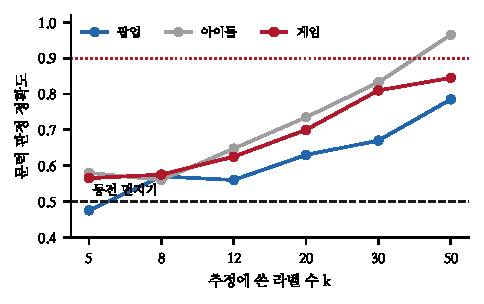
\includegraphics[width=\columnwidth]{figs/acc.pdf}
\caption{문턱 판정 정확도. k=8에서는 세 도메인 모두 동전 던지기다.}
\end{figure}

\begin{table}[t]
\centering\tsize
\caption{``참 r이 0.5를 넘는가''를 k건으로 맞히는 정확도.}
\begin{tabular}{lrrrrr}
\toprule
도메인 & 참 r & k=8 & k=20 & k=30 & k=50 \\
\midrule
아이돌 & $+$0.681 & 56\% & 74\% & 83\% & \textbf{96\%} \\
게임 & $+$0.344 & 57\% & 70\% & 81\% & 84\% \\
팝업 & $+$0.445 & 57\% & 63\% & 67\% & 78\% \\
\bottomrule
\end{tabular}
\end{table}

k=8에서 셋 다 56--57\%다. 동전을 던지는 것과 같다.

\claimx{순위 상관 추정은 여덟 건에서도 거의 편향이 없지만, 문턱 판정은 쉰 건이
있어야 80\% 이상 맞는다. 추정의 정확도와 판정의 정확도는 다른 문제다.}{문턱을
0.5가 아니라 도메인 참값에서 먼 곳(예: 0.3)에 두면 적은 k로도 판정할 수 있다.
문턱 위치를 바꿔 재보면 이 결론의 일반성을 알 수 있다.}

\paragraph{팝업이 가장 어렵다}
참값 $+$0.445가 문턱 0.5에 가장 가깝기 때문이다. k=50에서도 78\%에 그친다.
경계에 있는 값은 표본을 아무리 늘려도 판정이 어렵다 --- 이것은 추정의 문제가
아니라 문턱을 참값 근처에 둔 것의 문제다.

\section{비대칭이 절차를 바꾼다}

\begin{figure}[t]
\centering

\includegraphics[width=\columnwidth]{figs/cost.pdf}
\caption{같은 파이프라인 안에서 두 단계의 라벨 비용.}
\end{figure}

\begin{table}[t]
\centering\tsize
\caption{단계별 필요 라벨.}
\begin{tabular}{lrl}
\toprule
단계 & k & 무엇을 정하나 \\
\midrule
눈금 보정 & \textbf{8} & 중심과 중앙절대편차 두 모수 \\
문턱 판정 & \textbf{50} & 순위 상관이 0.5를 넘는가 \\
\bottomrule
\end{tabular}
\end{table}

여섯 배 차이다. 문턱을 사전에 확정하려면 눈금 보정보다 여섯 배 많은 실측이
필요하고, 그 정도면 ``쓸지 말지''를 정하는 데 ``쓰는 것''보다 비싼 값을 치르는
셈이다.

\paragraph{그러면 내부 모델을 쓰면 되지 않나}
50건이 있으면 그 도메인 자체로 모델을 만들 수 있을 것 같다. 그런데 노트 25가
그것을 막는다 --- 가용 피처 전부를 넣고 교차검증하면 팝업이 $-$10.6\%, 아이돌이
$-$10.4\%로 상수보다 나쁘다. 도메인당 표본이 작아 내부 학습이 되지 않는다.
전이는 여전히 옳은 접근이고, 다만 그 적합성을 싸게 판정할 방법이 없다.

\claimx{문턱 판정 비용이 눈금 보정 비용의 여섯 배이므로, 문턱을 사전 확정 조건으로
쓰면 안 된다.}{순위 상관을 라벨 없이 추정하는 방법(예: 출처 도메인 간 상관의
일관성으로 대리)이 나오면 이 비대칭이 사라진다.}

\section{그래서 절차를 이렇게 고친다}

\begin{enumerate}[leftmargin=1.3em,itemsep=0.2em]
\item 순위 전이가 순열 검정을 통과하는지 본다. \textbf{라벨 불필요.}
\item 통과하면 8--20건을 실측해 눈금을 잡고 절대량을 낸다.
\item 같은 8--20건으로 순위 상관을 \emph{추정만} 한다. 판정에 쓰지 않는다.
      추정치가 낮으면(0.3 미만) 결과를 보수적으로 읽는다.
\item 실측 건수가 50건을 넘어가면 그때 문턱을 판정하고 계속 쓸지 정한다.
\end{enumerate}

사전 게이트를 사후 점검으로 바꾼 것이다. 노트 31은 ``문턱 아래면 절대량 단계로
넘어가지 않는다''고 썼는데, 그 판정을 미리 할 수 없으므로 실행 순서를 뒤집는다.

\section{한계}

\begin{itemize}[leftmargin=1.1em,itemsep=0.15em]
\item 문턱 0.5는 노트 31에서 세 도메인 배치를 보고 그은 선이다. 이론적 근거가
      없으므로 이 노트의 판정 비용도 그 선에 딸려 있다.
\item 상관 추정에 피어슨을 썼다. 스피어만이나 축소 추정량에서는 표준편차가
      다를 수 있다.
\item k건은 무작위 추출을 가정한다. 노트 22에서 시간순 추출이 아이돌에서
      위험함을 보였는데, 상관 추정에서도 같을 수 있다.
\item 세 도메인 모두 참 r이 0.34--0.68 구간에 있다. 훨씬 높거나 낮은 도메인에서는
      판정이 쉬울 것이다.
\end{itemize}

\section{다음}

\begin{enumerate}[leftmargin=1.3em,itemsep=0.15em]
\item 라벨 없이 순위 상관을 대리 추정하는 방법 --- 이 비대칭을 없애는 유일한 길.
\item 입장 허들의 게임 측정 경로 --- 여러 노트째 미해결.
\item 네 번째 도메인.
\item 시간순 k건에서 상관 추정의 편향 확인.
\end{enumerate}

\vspace{0.6em}
\hrule height 0.3pt
\vspace{0.5em}
{\footnotesize
\textbf{참고문헌}\\[0.3em]
Fisher, R. A. (1915). Frequency distribution of the values of the correlation
coefficient in samples from an indefinitely large population.
\emph{Biometrika}, 10(4), 507--521.\\[0.15em]
Cohen, J. (1988). \emph{Statistical Power Analysis for the Behavioral Sciences},
2nd ed. Lawrence Erlbaum.\\[0.15em]
Efron, B., Tibshirani, R. (1993). \emph{An Introduction to the Bootstrap}.
Chapman \& Hall.\\[0.15em]
Ben-David, S. et al. (2010). A theory of learning from different domains.
\emph{Machine Learning}, 79(1--2), 151--175.
}

\end{document}
